
\documentclass[12pt,a4paper]{article}
\usepackage[margin=2.5cm]{geometry}
\usepackage{titling}
\usepackage{datetime2}
\usepackage{graphicx}
\usepackage{float}
\usepackage{amsmath}

\title{\textbf{Light Polarization Modulation Using a Liquid Crystal Cell:}\\
Detection of Malaria Pigment -- Magneto}

\author{
Nguyen Ba Phi (S3VYH3)\\
Mariana Uribe Unigarro (IE5SG5)
}

\date{\today}

\begin{document}

\maketitle





\section{Abstract}
The aim of this laboratory experiment was to investigate light
polarization modulation using a voltage-controlled liquid crystal
(LC) cell and to study the magneto-optical detection of hemozoin
crystals, which are associated with malaria infection. It also
investigated how magnetic fields and hemozoin concentration affect
the detected optical signal. The polarizer measurements gave a
maximum voltage of \(1504\,\mathrm{mV}\) and a minimum of
\(2\,\mathrm{mV}\). The LC cell and measurement system were also
tested, and the final measurements examined changes in the signal
under different experimental conditions.







\section{Introduction}

Light polarization describes the orientation of the oscillating
electric field of an electromagnetic wave. When linearly polarized
light passes through a polarizer, only the electric-field component
parallel to the transmission axis is transmitted. Therefore,
the transmitted intensity depends on the relative orientation of
the polarizers and follows Malus' law for ideal polarizers.

In materials whose optical properties depend on the direction in which light travels or the direction in which its electric field oscillates, a phase difference between orthogonal components of the electric field can be introduced. This is known as birefringe and it allows the polarization state of the light to be modified without changing its propagation direction. Liquid crystals such as the one worked in this laboratory, have a controllable birefringence because their molecular orientation can be modified
by an applied electric field. Therefore, an LC cell can function
as a voltage-controlled optical retarder.

In this experiment, film polarizers and a liquid crystal cell
were used to characterize polarization-dependent transmission
and develop a polarization-modulation measurement system. A
photodetector and lock-in amplifier were later used to
investigate the response of hemozoin suspensions under different
magnetic-field orientations and concentrations.








\section{Measurement Tools}

The following equipment was used during the experiment:

\begin{itemize}
    \item \textbf{Analog Discovery 3 (Digilent AD3):}
    Used as a waveform generator, oscilloscope, and lock-in amplifier.
    The WaveForms software was used for communication and data acquisition.

    \item \textbf{Signal Generator (Siglent SDG1062X):}
    Used to generate electrical signals.

    \item \textbf{Laser Diode:}
    A laser with a wavelength of \(650\,\mathrm{nm}\).

    \item \textbf{Rotatable Film Polarizers:}
    Used to control the polarization direction of light.

    \item \textbf{Liquid Crystal Cell (Thorlabs LCC1111U-A):}
    Mounted on a rotatable holder and used to modify light polarization.

    \item \textbf{Sample Holder with Rotatable Magnet:}
    Included a \(20\,\mathrm{mm}\) cuvette for holding the hemozoin suspension. The following three sample configurations were used:
    \begin{itemize}
        \item A sample holder with 0\% hemozoin, meaning that it is empty and contains only air.
        \item A sample holder with 5\% hemozoin suspension in water.
        \item A sample holder with 10\% hemozoin suspension in water.
    \end{itemize}

    \item \textbf{Photodetector:}
    Used to measure the transmitted light signal.
\end{itemize}











\subsection{Task 1: Basic Characterization of Film Polarizers}

\textbf{Objective.}
The aim of this task was to determine the angular dependence of transmitted light intensity, verify Malus' law, identify the parallel and perpendicular orientations of the polarizers, and calculate their extinction ratio.


\textbf{Procedure.}
The laser diode and photodetector were aligned along the optical rail. The first polarizer was placed and rotated such that the transmitted intensity was maximized before adding the analyzer (second polarizer). With both polarizers in place (See Figure~\ref{fig:setup_image}), the analyzer was rotated in steps of \(10^\circ\), and the detector voltage was recorded at each angle. The background voltage caused by room illumination was measured as \(21\,\mathrm{mV}\) and subtracted from each measurement. \cite{lab_desc}

The corrected voltage was plotted as a function of analyzer
angle (See Figure~\ref{fig:t1_correctedV_vs_angle}). For ideal polarizers, Malus' law:
\begin{equation}
I(\theta)=I_{\max}
\cos^2(\theta-\theta_{\parallel}),
\end{equation}
where \(\theta_{\parallel}\) is the angle at which the
polarizers are parallel.



\begin{figure}[H]
    \centering
    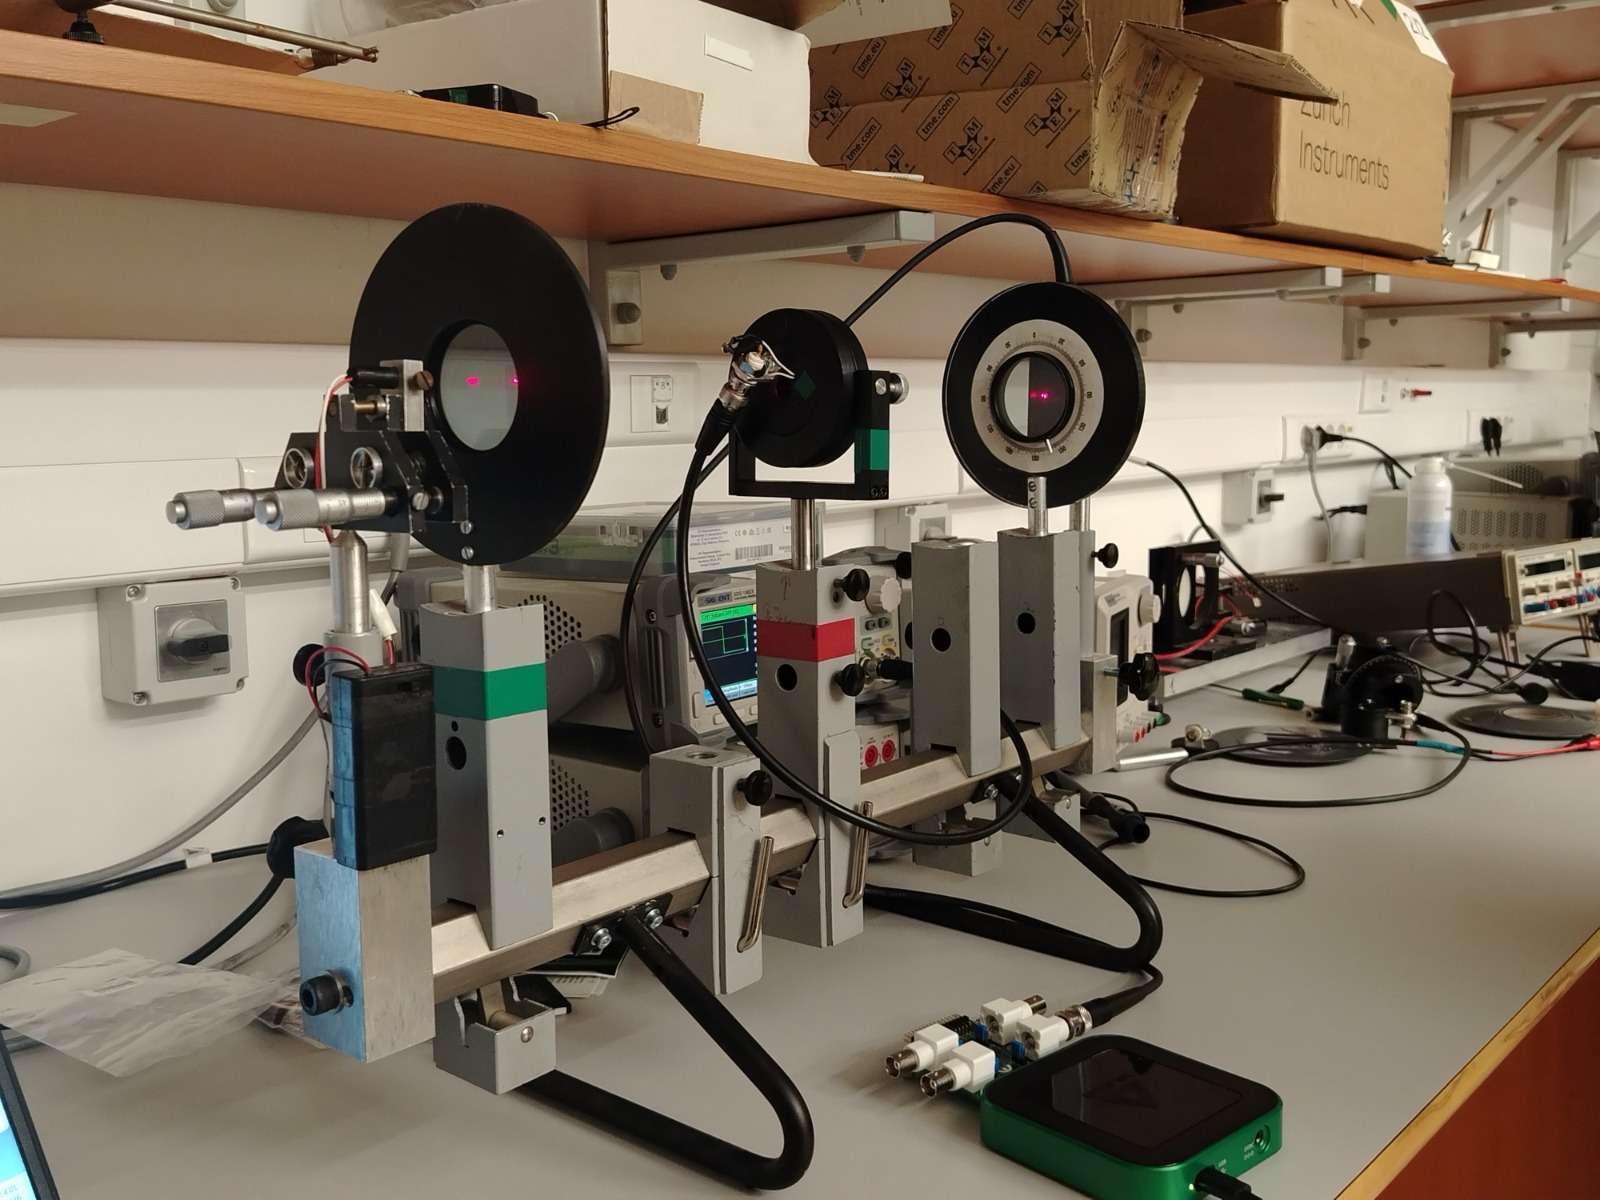
\includegraphics[width=0.7\linewidth]{WhatsApp Image 2026-10-10 at 20.13.14.jpeg}
    \caption{Initial Set Up}
    \label{fig:setup_image}
\end{figure}



\textbf{Results}

The maximum corrected voltage was \(1504\,\mathrm{mV}\)
at \(140^\circ\), corresponding to the parallel reference
orientation. The minimum was \(2\,\mathrm{mV}\) at
\(60^\circ\), approximately \(80^\circ\) from the parallel
reference orientation.

The general measurement uncertainties for the angular positions were estimated as \(\pm 3^\circ\) for the rotatable film polarizers and \(\pm 1^\circ\) for the LC cell rotation mount. For the voltage readings, it was observed that the measurement error is non-constant and depends on the magnitude of the measured signal, with smaller absolute errors occurring at smaller voltages.

The extinction ratio was calculated as
\begin{equation}
ER=\frac{I_{\perp}}{I_{\parallel}}
\approx\frac{U_{\perp}}{U_{\parallel}}
=\frac{2}{1504}\approx 0.00133.
\end{equation}

Because the voltage uncertainty scales non-linearly with the signal magnitude, applying a uniform overall error estimate (such as an averaged \(\pm 8\,\mathrm{mV}\)) would heavily overestimate the uncertainty of the very small minimum transmission reading (\(U_{\perp} = 2\,\mathrm{mV}\)). Consequently, a standard variance-based error propagation using a constant voltage error would be inaccurate and has been omitted here.

The extinction ratio quantifies the efficiency of the polarizers, representing the fraction of light that leaks through when they are perfectly crossed compared to when they are parallel. Our result of approximately \(1.33 \times 10^{-3}\) (or 1:750) aligns reasonably well with commercial standards. For comparison, standard commercial dichroic film polarizers (such as economy models from Thorlabs) typically feature extinction ratios ranging from \(>1000:1\) (\(10^{-3}\)) to \(>5000:1\) in the visible spectrum.\cite{thorlabs_film_polarizers}

The measurements show a clear angular dependence of transmission,
consistent with the expected behavior of polarizers



\begin{figure}[H]
    \centering
    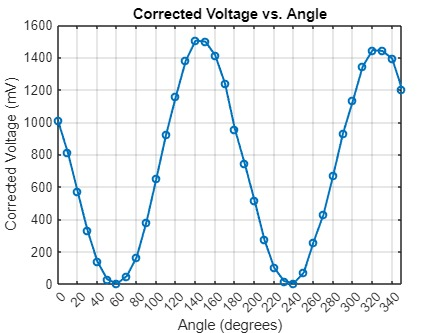
\includegraphics[width=0.7\linewidth]{WhatsApp Image 2026-10-10 at 20.02.04.jpeg}
    \caption{Corrected Voltage vs Angle. The corrected voltage represents the measured photodetector voltage minus the \(21\,\mathrm{mV}\) background illumination. The angle corresponds to the absolute angular scale displayed on the analyzer's mount, rather than the relative angle to the first polarizer.}
    \label{fig:t1_correctedV_vs_angle}
\end{figure}








\subsection{Task 2: Polarization State After the LC Cell}

\textbf{Objective.}
The goal of this task was to investigate the polarization state of light after transmission through an LC cell whose optical axis is oriented at \(45^\circ\) relative to the first polarizer.

\textbf{Procedure.}
The experimental setup, as shown previously in Figure~\ref{fig:setup_image}, included the LC cell positioned between the two polarizers. First, the two polarizers were set parallel. The LC cell was then inserted and rotated until the transmitted intensity was maximized, indicating that its optical axis was parallel to the polarizers, and this initial angle was noted. 

Theoretically, the second step was to set the polarizers perpendicular and rotate the LC cell again to maximize intensity, which should correspond to a \(45^\circ\) shift. However, instead of performing this second step experimentally, the LC cell was simply manually rotated by \(45^\circ\) from its initial position. The analyzer was then rotated in steps of \(10^\circ\), and the photodetector voltage was recorded. The background voltage of \(21\,\mathrm{mV}\) was subtracted from each measurement.

\begin{figure}[H]
    \centering
    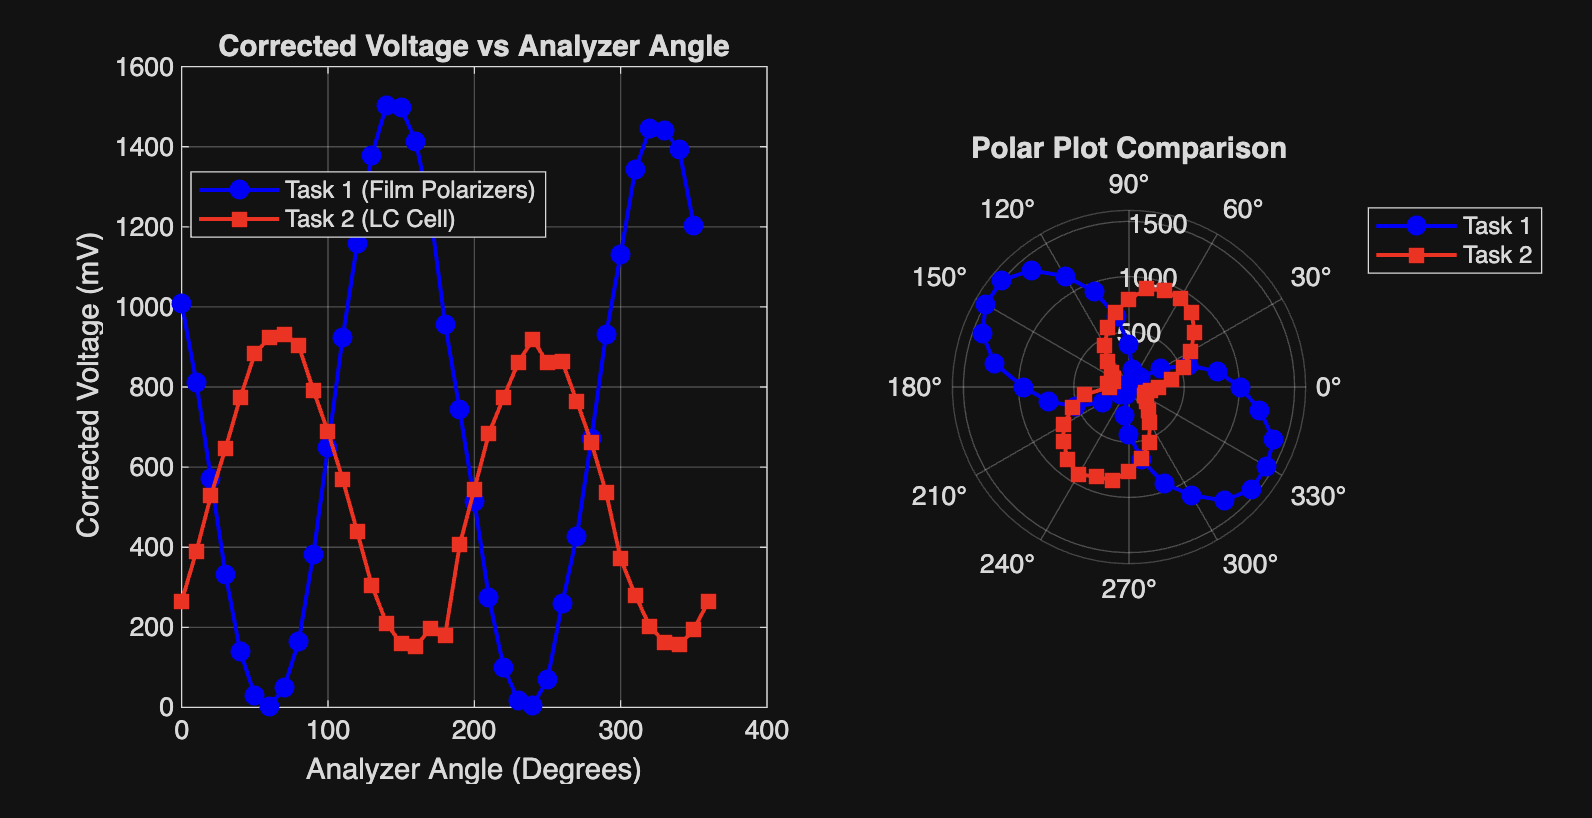
\includegraphics[width=0.9\linewidth]{t2_polar_plot.png}
    \caption{Corrected Voltage vs Analyzer Angle (left) and Polar Plot comparison of Task 1 and Task 2 (right). Task 1 (blue) shows the transmission of the polarizers alone, while Task 2 (red) shows the transmission after the insertion of the zero-voltage LC cell. The average voltage dropped from $\approx 753$ mV to $\approx 541$ mV, The peak-to-peak amplitude compressed from $\approx 1502$ mV to $\approx 778$ mV}
    \label{fig:task2_results}
\end{figure}


\textbf{Results}
During the initial alignment with parallel polarizers, the LC cell angle that maximized intensity was found to be \(53^\circ\). After manually rotating the LC cell by \(45^\circ\) to \(98^\circ\), the analyzer rotation measurements were taken. 

Upon plotting the data (See Figure \ref{fig:task2_results}), significant changes in the transmission profile were observed compared to Task 1. First, the insertion of the LC cell introduced optical losses; the average corrected voltage dropped from approximately \(753\,\mathrm{mV}\) to \(541\,\mathrm{mV}\), and the peak-to-peak amplitude decreased from \(1502\,\mathrm{mV}\) to \(778\,\mathrm{mV}\). 

More importantly, the transmission curve exhibited a distinct angular shift. The maximum intensity shifted from \(140^\circ\) in Task 1 to \(70^\circ\) in Task 2. While the lab supervisors initially suggested this indicated a technical problem (likely because the cell did not hit an ideal \(\pi/2\) quarter-wave circular polarization state at zero voltage), the smooth and continuous nature of the data clearly maps an elliptical polarization state. The cell was functioning as a waveplate, just with a non-ideal baseline retardation.

We can confidently extract this zero-voltage retardation, \(\delta\), by evaluating the transmitted intensities at the parallel (\(\theta_{\parallel} = 140^\circ\)) and perpendicular (\(\theta_{\perp} = 50^\circ\)) positions. The measured corrected voltages at these angles were \(V_{\parallel} = 210\,\mathrm{mV}\) and \(V_{\perp} = 883\,\mathrm{mV}\). 

Normalizing these values against the total intensity along the principal axes (\(I_{total} = 210 + 883 = 1093\,\mathrm{mV}\)) gives the normalized transmissions:
\begin{equation}
T_{\parallel} = \frac{210}{1093} \approx 0.192 \quad \text{and} \quad T_{\perp} = \frac{883}{1093} \approx 0.808
\end{equation}

For an LC cell at \(45^\circ\), the normalized transmission through parallel polarizers is defined as \(T_{\parallel} = \cos^2\left(\frac{\delta}{2}\right)\). Using our normalized \(T_{\parallel}\), the zero-voltage retardation can be calculated as:
\begin{equation}
\delta = 2 \arccos\left(\sqrt{0.192}\right) \approx 2.23\,\mathrm{rad} \approx 128^\circ
\end{equation}

With the retardation known, the optical path-length difference, \(\Delta n d\), can be determined using the phase shift relationship \(\delta = \frac{2\pi}{\lambda} \Delta n d\). Given the laser diode wavelength of \(\lambda = 650\,\mathrm{nm}\), the path-length difference is:
\begin{equation}
\Delta n d = \frac{\delta \cdot \lambda}{2\pi} = \frac{2.23 \cdot 650\,\mathrm{nm}}{2\pi} \approx 231\,\mathrm{nm}
\end{equation}











\subsection{Task 3: LC Retardation with Parallel Polarizers}

\textbf{Objective.}
The goal of this task was to investigate the voltage dependence of the optical retardation, \(\delta(V)\), of the liquid crystal cell using parallel polarizers.

\textbf{Procedure.}
The two polarizers were set parallel, and the LC cell was positioned with its optical axis at approximately \(45^\circ\) relative to the polarizer. 

Instead of increasing the RMS voltage step by step, a continuous acquisition method was utilized. A \(2\,\mathrm{kHz}\) rectangular AC signal was applied to the LC cell, and its amplitude was modulated using a triangle sweep from the signal generator. The sweep was set with a period of \(500\,\mathrm{ms}\) (\(2\,\mathrm{Hz}\)), producing a time-dependent detector signal. 

This raw time-domain data was subsequently post-processed. The relevant period was truncated, and the time axis was converted back to the corresponding RMS modulation input voltage to obtain the voltage-dependent transmission curve.

Based on Equation I.2.3 from the laboratory description \cite{lab_desc}, for an LC cell oriented at \(45^\circ\), the ideal normalized transmission through parallel polarizers is defined as:
\begin{equation}
T_{\parallel}=\cos^2\left(\frac{\delta}{2}\right).
\end{equation}

The retardation can therefore be estimated from the normalized transmission as:
\begin{equation}
\delta(V)=2\arccos\sqrt{T_{\parallel}(V)}.
\end{equation}


\textbf{Results.}
The raw time-domain signal (Figure~\ref{fig:task3_signals}a) was truncated to a single modulation period and mapped to the corresponding RMS voltage sweep (\(0.3\) to \(2.3\,V_\mathrm{rms}\)). The detector voltage decreased from \(1.12\,\mathrm{V}\) at \(0.3\,V_\mathrm{rms}\) to a minimum of \(0.02\,\mathrm{V}\) at \(1.9\,V_\mathrm{rms}\), before rising to a stable \(0.24\,\mathrm{V}\) (Figure~\ref{fig:task3_signals}b). 


\begin{figure}[H]
    \centering
    \begin{minipage}{0.48\textwidth}
        \centering
        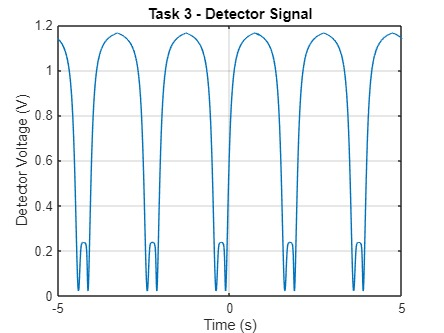
\includegraphics[width=\linewidth]{WhatsApp Image 2026-10-10 at 20.37.07.jpeg}
        \caption*{a) Detector Signal vs Time}
    \end{minipage}\hfill
    \begin{minipage}{0.48\textwidth}
        \centering
        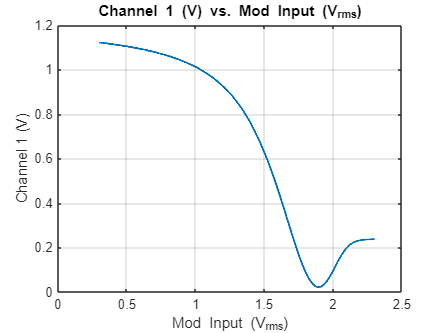
\includegraphics[width=\linewidth]{image.png}
        \caption*{b) Channel 1 vs Mod Input RMS}
    \end{minipage}
    \caption{LC Cell Retardation with parallel polarizers. The raw time-dependent detector signal (a) was truncated and converted to extract the voltage-dependent transmission profile (b).}
    \label{fig:task3_signals}
\end{figure}


After normalizing the signal against the dark level (\(0.02\,\mathrm{V}\)) and the maximum raw trace (\(1.17\,\mathrm{V}\)), the retardation \(\delta\) was calculated assuming a monotonic decrease with voltage (Figure~\ref{fig:task3_retardation}). The retardation dropped from \(\approx 1.9\pi\) at \(0.3\,V_\mathrm{rms}\) to \(\pi\) at \(1.9\,V_\mathrm{rms}\), flattening out at \(0.7\pi\) at \(2.3\,V_\mathrm{rms}\). 

This profile confirms the expected behavior of a nematic LC cell. At low voltages, the molecules are pinned by the alignment layers and retardation barely changes. Above a threshold, they tilt rapidly toward the field, causing \(\delta\) to drop. The transmission minimum at \(1.9\,V_\mathrm{rms}\) corresponds exactly to \(\delta=\pi\), where the cell acts as a half-wave plate and rotates the polarization by \(90^\circ\). The retardation never reaches zero because the molecules immediately adjacent to the alignment layers remain pinned, leaving a residual phase shift.

\begin{figure}[H]
    \centering
    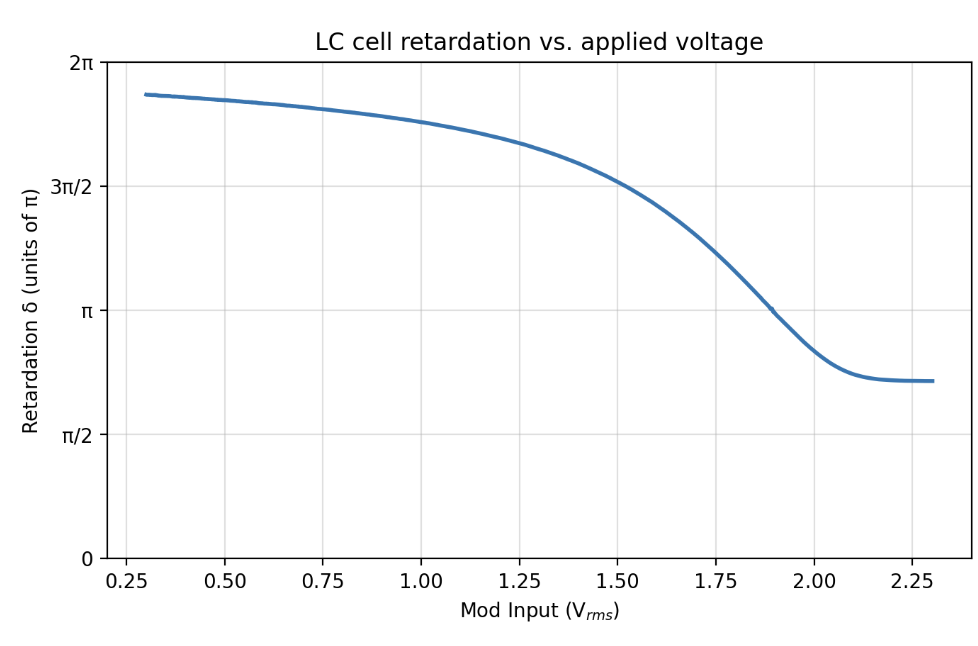
\includegraphics[width=0.5\linewidth]{t3_retardation_vs_voltage_parallel.png}
    \caption{Retardation \(\delta\) of the LC cell as a function of RMS voltage, calculated from the transmission with parallel polarizers.}
    \label{fig:task3_retardation}
\end{figure}







\subsection{Task 4: LC Retardation with Crossed Polarizers}

\textbf{Objective.}
The goal of this task was to investigate the voltage dependence of LC retardation with the analyzer perpendicular to the first polarizer.

\textbf{Procedure.}
The experimental procedure from Task 3 was repeated with the polarizers set perpendicular to one another. The same continuous acquisition method was utilized, applying a \(2\,\mathrm{kHz}\) rectangular AC signal modulated by a \(500\,\mathrm{ms}\) (\(2\,\mathrm{Hz}\)) triangle sweep to the LC cell. The raw time-dependent detector output was recorded and subsequently converted to plot against the RMS modulation input voltage.

Based on Equation I.2.4 from the laboratory description \cite{lab_desc}, for an LC cell oriented at \(45^\circ\), the ideal normalized transmission between crossed polarizers is:
\begin{equation}
T_{\perp}=\sin^2\left(\frac{\delta}{2}\right).
\end{equation}

The corresponding retardation can be estimated from:
\begin{equation}
\delta(V)=2\arcsin\sqrt{T_{\perp}(V)}.
\end{equation}

The parallel and crossed configurations complement one another; ideally, \(T_{\parallel}+T_{\perp}=1\). In the actual experiment, background light, imperfect polarizers, and other optical losses were taken into account before comparing the transmission curves.


\textbf{Results.}
Post-processing mirrored the methodology of Task 3. Figure~\ref{fig:task4_signals} shows the raw signal and the truncated curve mapped to the \(0.3\)--\(2.3\,V_\mathrm{rms}\) sweep. The detector voltage was normalized between the dark level and the maximum of the trace to obtain \(T_\perp\). 


\begin{figure}[H]
    \centering
    \begin{minipage}{0.48\textwidth}
        \centering
        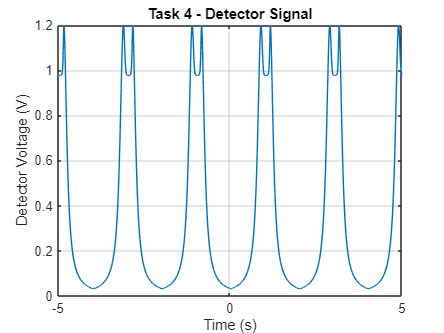
\includegraphics[width=\linewidth]{4.png}
        \caption*{a) Detector Signal vs Time}
    \end{minipage}\hfill
    \begin{minipage}{0.48\textwidth}
        \centering
        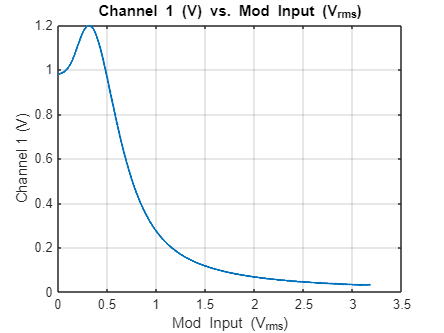
\includegraphics[width=\linewidth]{4.2.png}
        \caption*{b) Channel 1 vs Mod Input RMS}
    \end{minipage}
    \caption{LC Cell Retardation with crossed polarizers. The raw time-dependent detector signal (a) was truncated and converted to extract the voltage-dependent transmission profile (b).}
    \label{fig:task4_signals}
\end{figure}


Figure~\ref{fig:task4_T} plots \(T_\perp\) alongside the \(T_\parallel\) data from Task 3. The curves demonstrate the expected complementary relationship. \(T_\perp\) rises from \(0.03\) at \(0.3\,V_\mathrm{rms}\) to a maximum of \(\approx 1\) at \(1.9\,V_\mathrm{rms}\), before settling at \(0.81\). Conversely, \(T_\parallel\) goes from \(0.96\) to \(0\) and then to \(0.19\). On average, the sum of the two configurations is \(T_\parallel+T_\perp \approx 0.98\), closely matching theoretical expectations.


\begin{figure}[H]
    \centering
    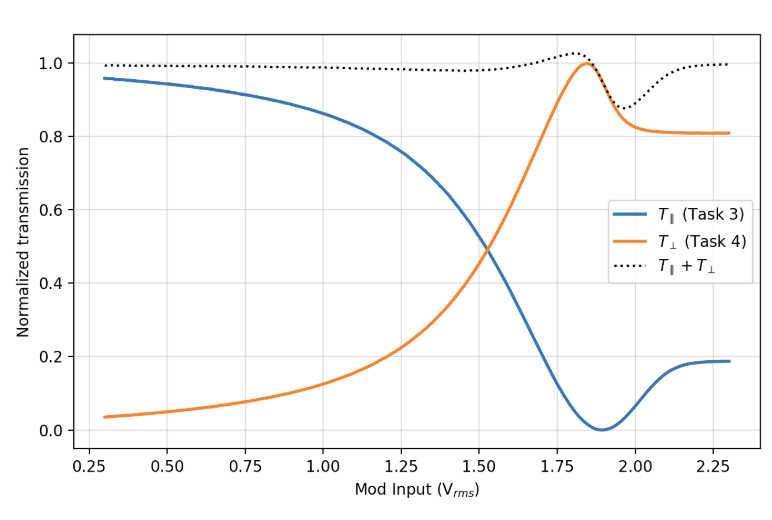
\includegraphics[width=0.6\linewidth]{retardation_comparison.png}
    \caption{Normalized transmission with parallel (\(T_\parallel\), Task 3) and crossed (\(T_\perp\), Task 4) polarizers as a function of RMS voltage. The dotted line shows \(T_\parallel+T_\perp\).}
    \label{fig:task4_T}
\end{figure}

The retardation was extracted from the crossed-polarizer transmission as \(\delta=2\arcsin\sqrt{T_\perp}\) (Figure~\ref{fig:task4_delta}). It falls from \(\approx 1.9\pi\) at \(0.3\,V_\mathrm{rms}\) to \(\pi\) at \(1.9\,V_\mathrm{rms}\), flattening out at \(0.7\pi\) above \(2.2\,V_\mathrm{rms}\). This aligns perfectly with the Task 3 calculations, further verifying the threshold and pinning dynamics of the LC cell. The half-wave point (\(T_\perp=1\), \(T_\parallel=0\)) confirms the voltage at which the cell successfully rotates the polarization by \(90^\circ\).


\begin{figure}[H]
    \centering
    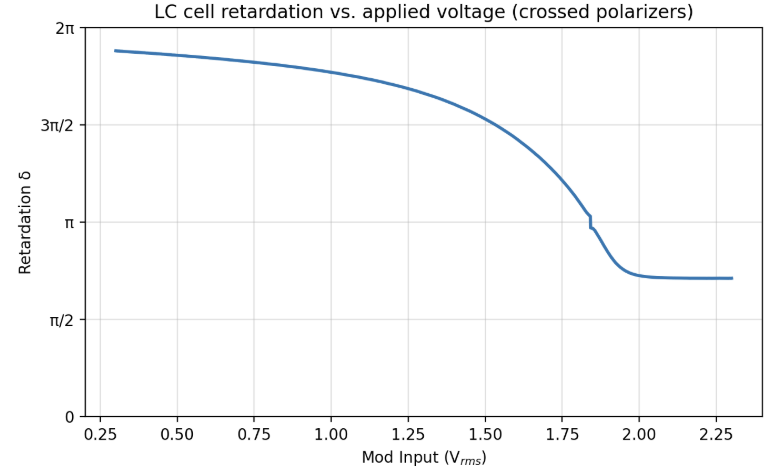
\includegraphics[width=0.6\linewidth]{t4_retardation_vs_voltage_perp.png}
    \caption{Retardation \(\delta\) of the LC cell as a function of RMS voltage, calculated from the transmission with crossed polarizers.}
    \label{fig:task4_delta}
\end{figure}










\section {Part 2}
\subsection{Task 5: Calibration of the Linear Dichroism Measurement}

\textbf{Objective.}
The goal of this task was to calibrate the polarization-modulation setup by measuring the detector's DC response and the second-harmonic lock-in signal as the analyzer angle was varied. The objective was also to compare modulation settings and select a suitable operating condition for the hemozoin measurements.

\textbf{Procedure.}
The setup consisted of placing the LC cell between the polarizers, with the analyzer positioned near \(45^\circ\) relative to the first polarizer. Small changes in the angle were introduced around this position. The LC modulation signal was adjusted to minimize the unwanted first-harmonic component, and the lock-in amplifier was configured to measure the second harmonic.

The characteristic square-wave voltage recorded in the notes was \(1.15\pm0.05\,\mathrm{V_{pp}}\). Calibration measurements were then performed under three different settings from the waveform generator: \(200\,\mathrm{mV}\) at \(20\,\mathrm{Hz}\), \(500\,\mathrm{mV}\) at \(20\,\mathrm{Hz}\), and \(200\,\mathrm{mV}\) at \(69\,\mathrm{Hz}\).

The detector and lock-in responses were plotted against the analyzer angle. Linear regression was used to determine sensitivity from the slope of each calibration curve. The coefficient of determination, \(R^2\), was used to assess the linearity of the measured response.

The sensitivity was calculated using:
\begin{equation}
S=\frac{\Delta U}{\Delta\theta},
\end{equation}
where \(U\) represents the detector or lock-in output and \(\theta\) is the analyzer angle.

\textbf{Results}
The measured calibration results are summarized in Table~\ref{tab:calibration}.

\begin{table}[H]
\centering
\caption{Calibration sensitivities and coefficients of determination.}
\label{tab:calibration}
\begin{tabular}{lcccc}
\hline
Setting &
\shortstack{Detector\\sensitivity} &
\(R^2\) &
\shortstack{Lock-in\\sensitivity} &
\(R^2\) \\
\hline
200 mV, 20 Hz & 5.12 & 0.9949 & 0.1042 & 0.7057 \\
500 mV, 20 Hz & 5.50 & 1.0000 & 0.4650 & 0.9153 \\
200 mV, 69 Hz & 5.25 & 0.9992 & 0.2025 & 0.6911 \\
\hline
\end{tabular}

\vspace{2mm}
\footnotesize
Detector sensitivity is expressed in \(\mathrm{mV/degree}\) and lock-in
sensitivity in \(\mu\mathrm{V/degree}\).
\end{table}

For the first setting (200 mV, 20 Hz), the lock-in maximum-output calibration demonstrated an exceptional sensitivity of \(0.0866\,\mathrm{mV/degree}\) (equivalent to \(86.6\,\mu\mathrm{V/degree}\)) with a highly linear fit (\(R^2=0.9940\)).

The detector response was highly linear under all three conditions. While the lock-in response showed some variation, it is important to note that increasing the modulation amplitude (such as the \(500\,\mathrm{mV}\) setting) can introduce unwanted first-harmonic components that degrade the purity of the second-harmonic lock-in signal. 

When factoring in the maximum-output calibration and the need to minimize non-linear harmonic noise, the \(200\,\mathrm{mV}\), \(20\,\mathrm{Hz}\) configuration provided the most stable and sensitive clean signal. Based on this optimal balance of high sensitivity and linearity, \(200\,\mathrm{mV}\) at \(20\,\mathrm{Hz}\) was selected as the operating condition for the subsequent hemozoin measurements.

\begin{figure}[H]
    \centering
    \begin{minipage}{0.5\textwidth}
        \centering
        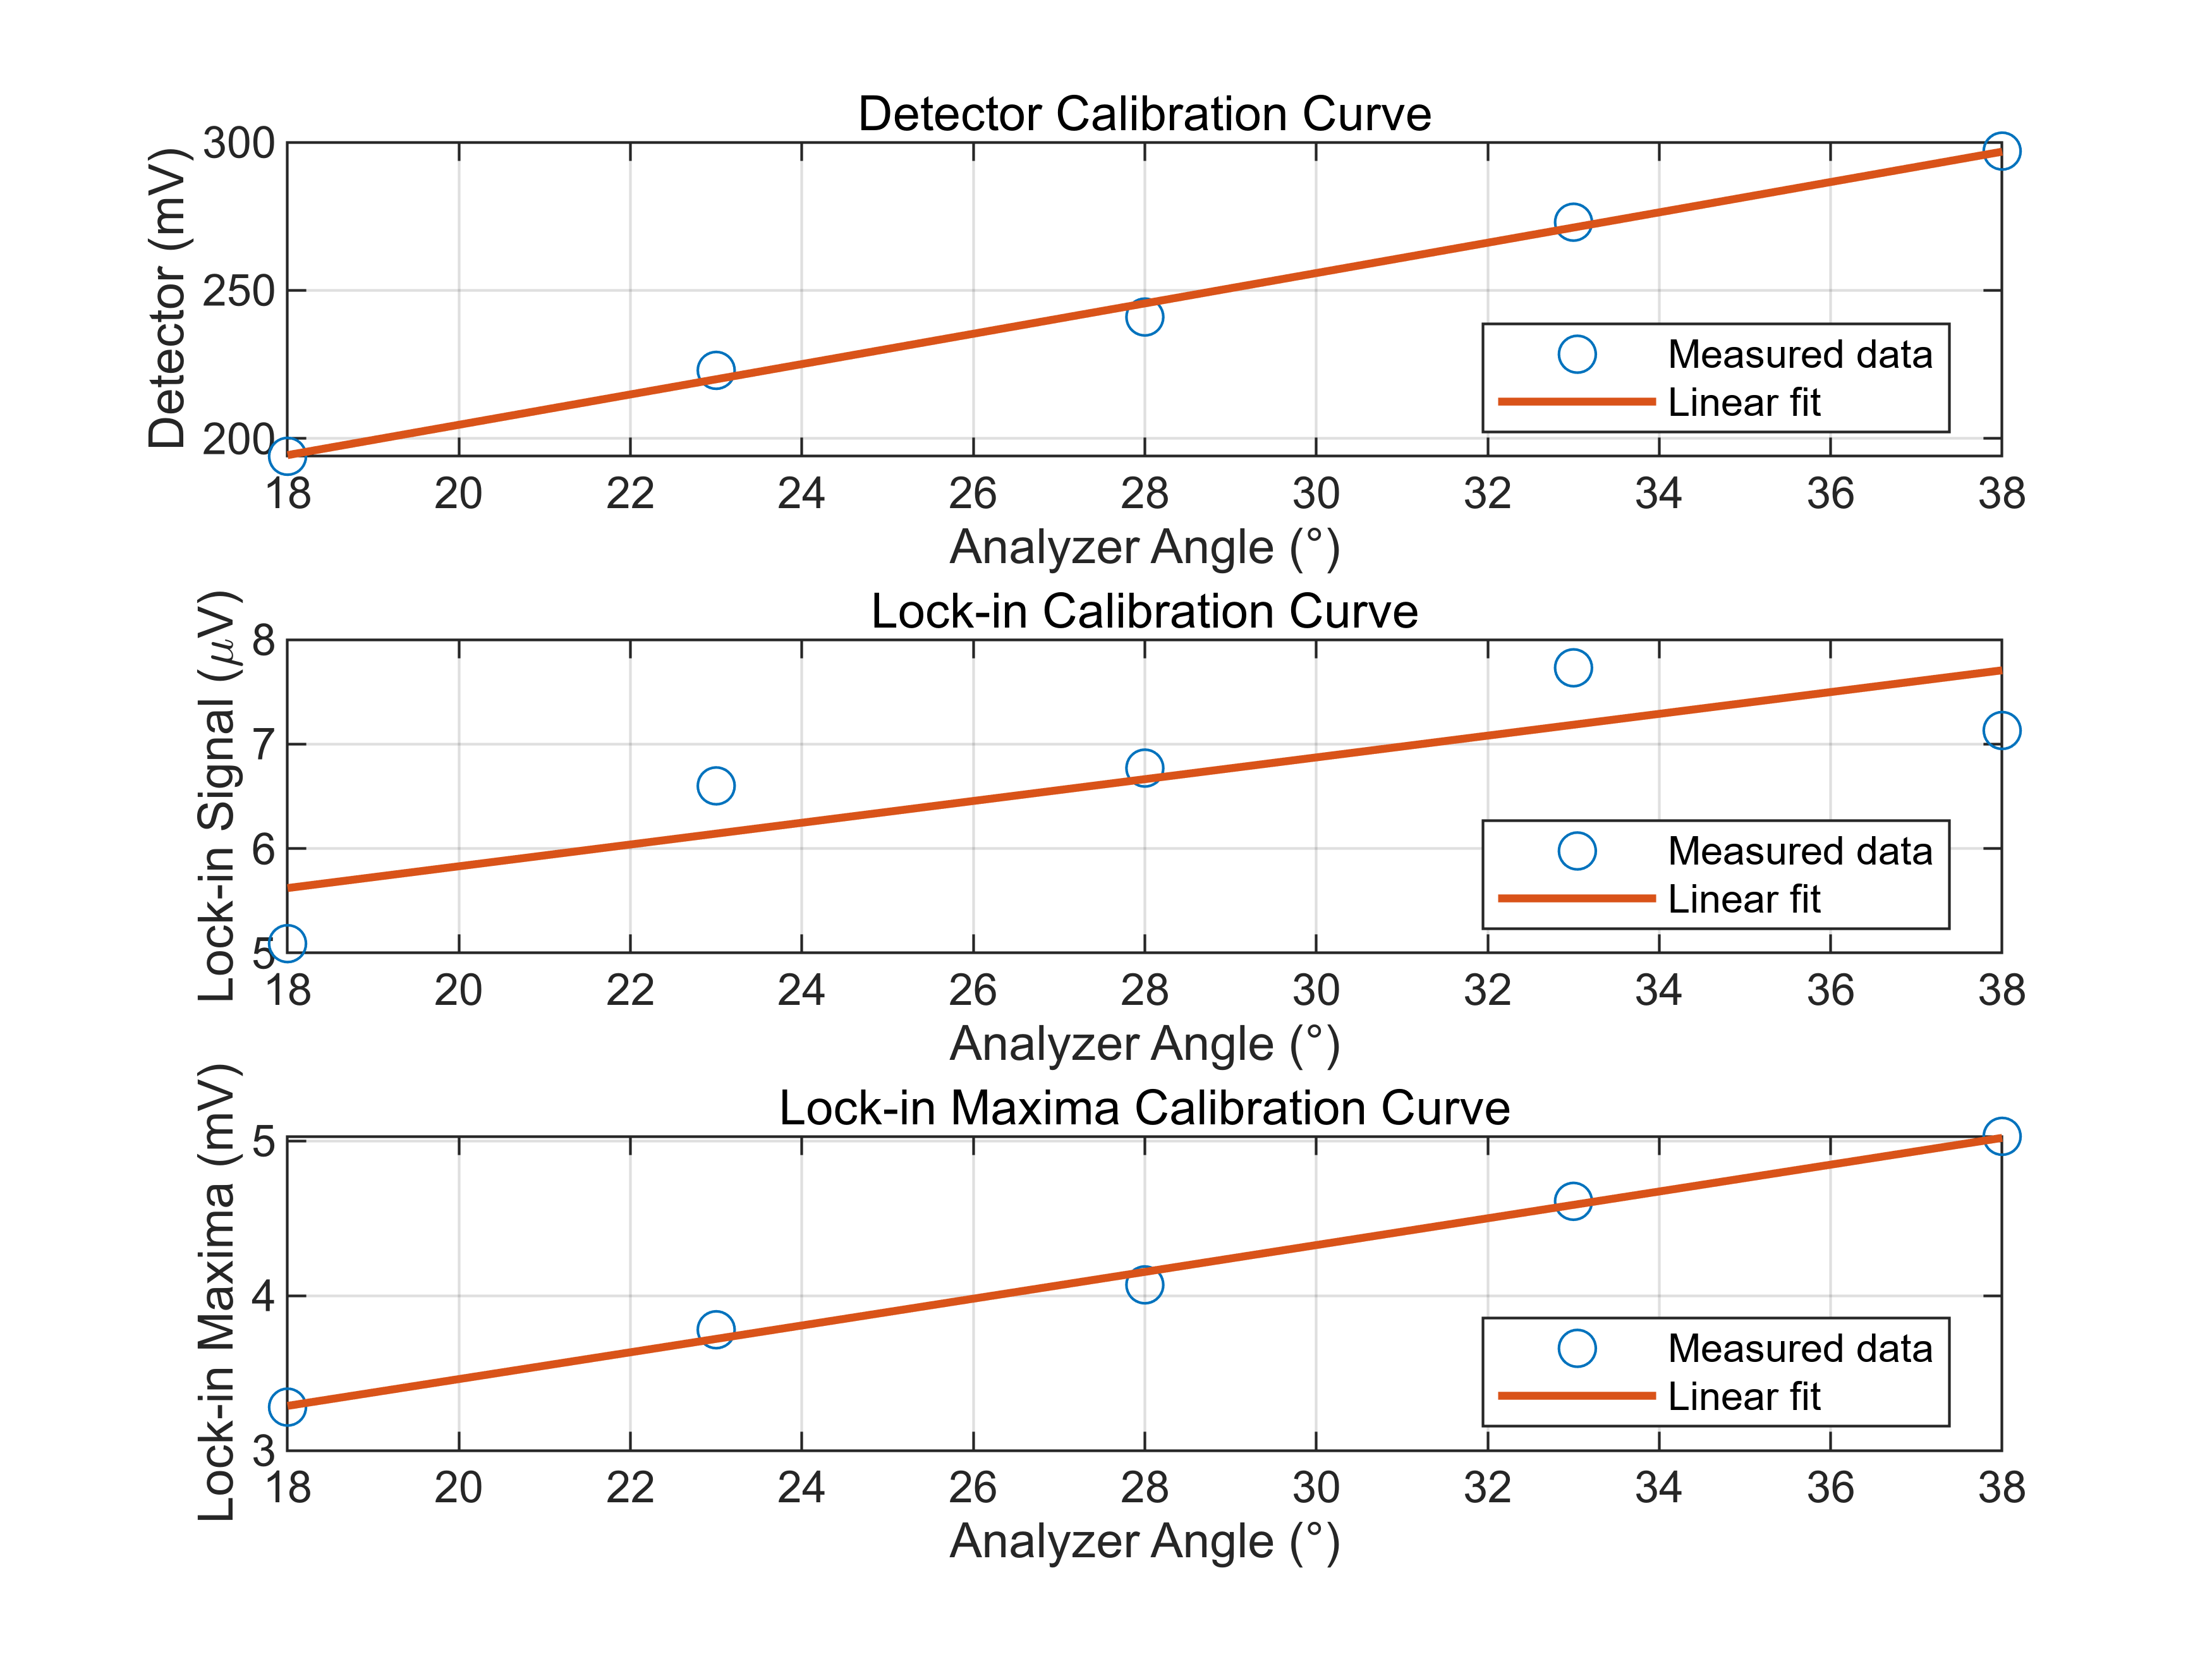
\includegraphics[width=\linewidth]{5.1.png}
        \caption*{a) 200 mV, 20 Hz}
    \end{minipage}\hfill
    \begin{minipage}{0.5\textwidth}
        \centering
        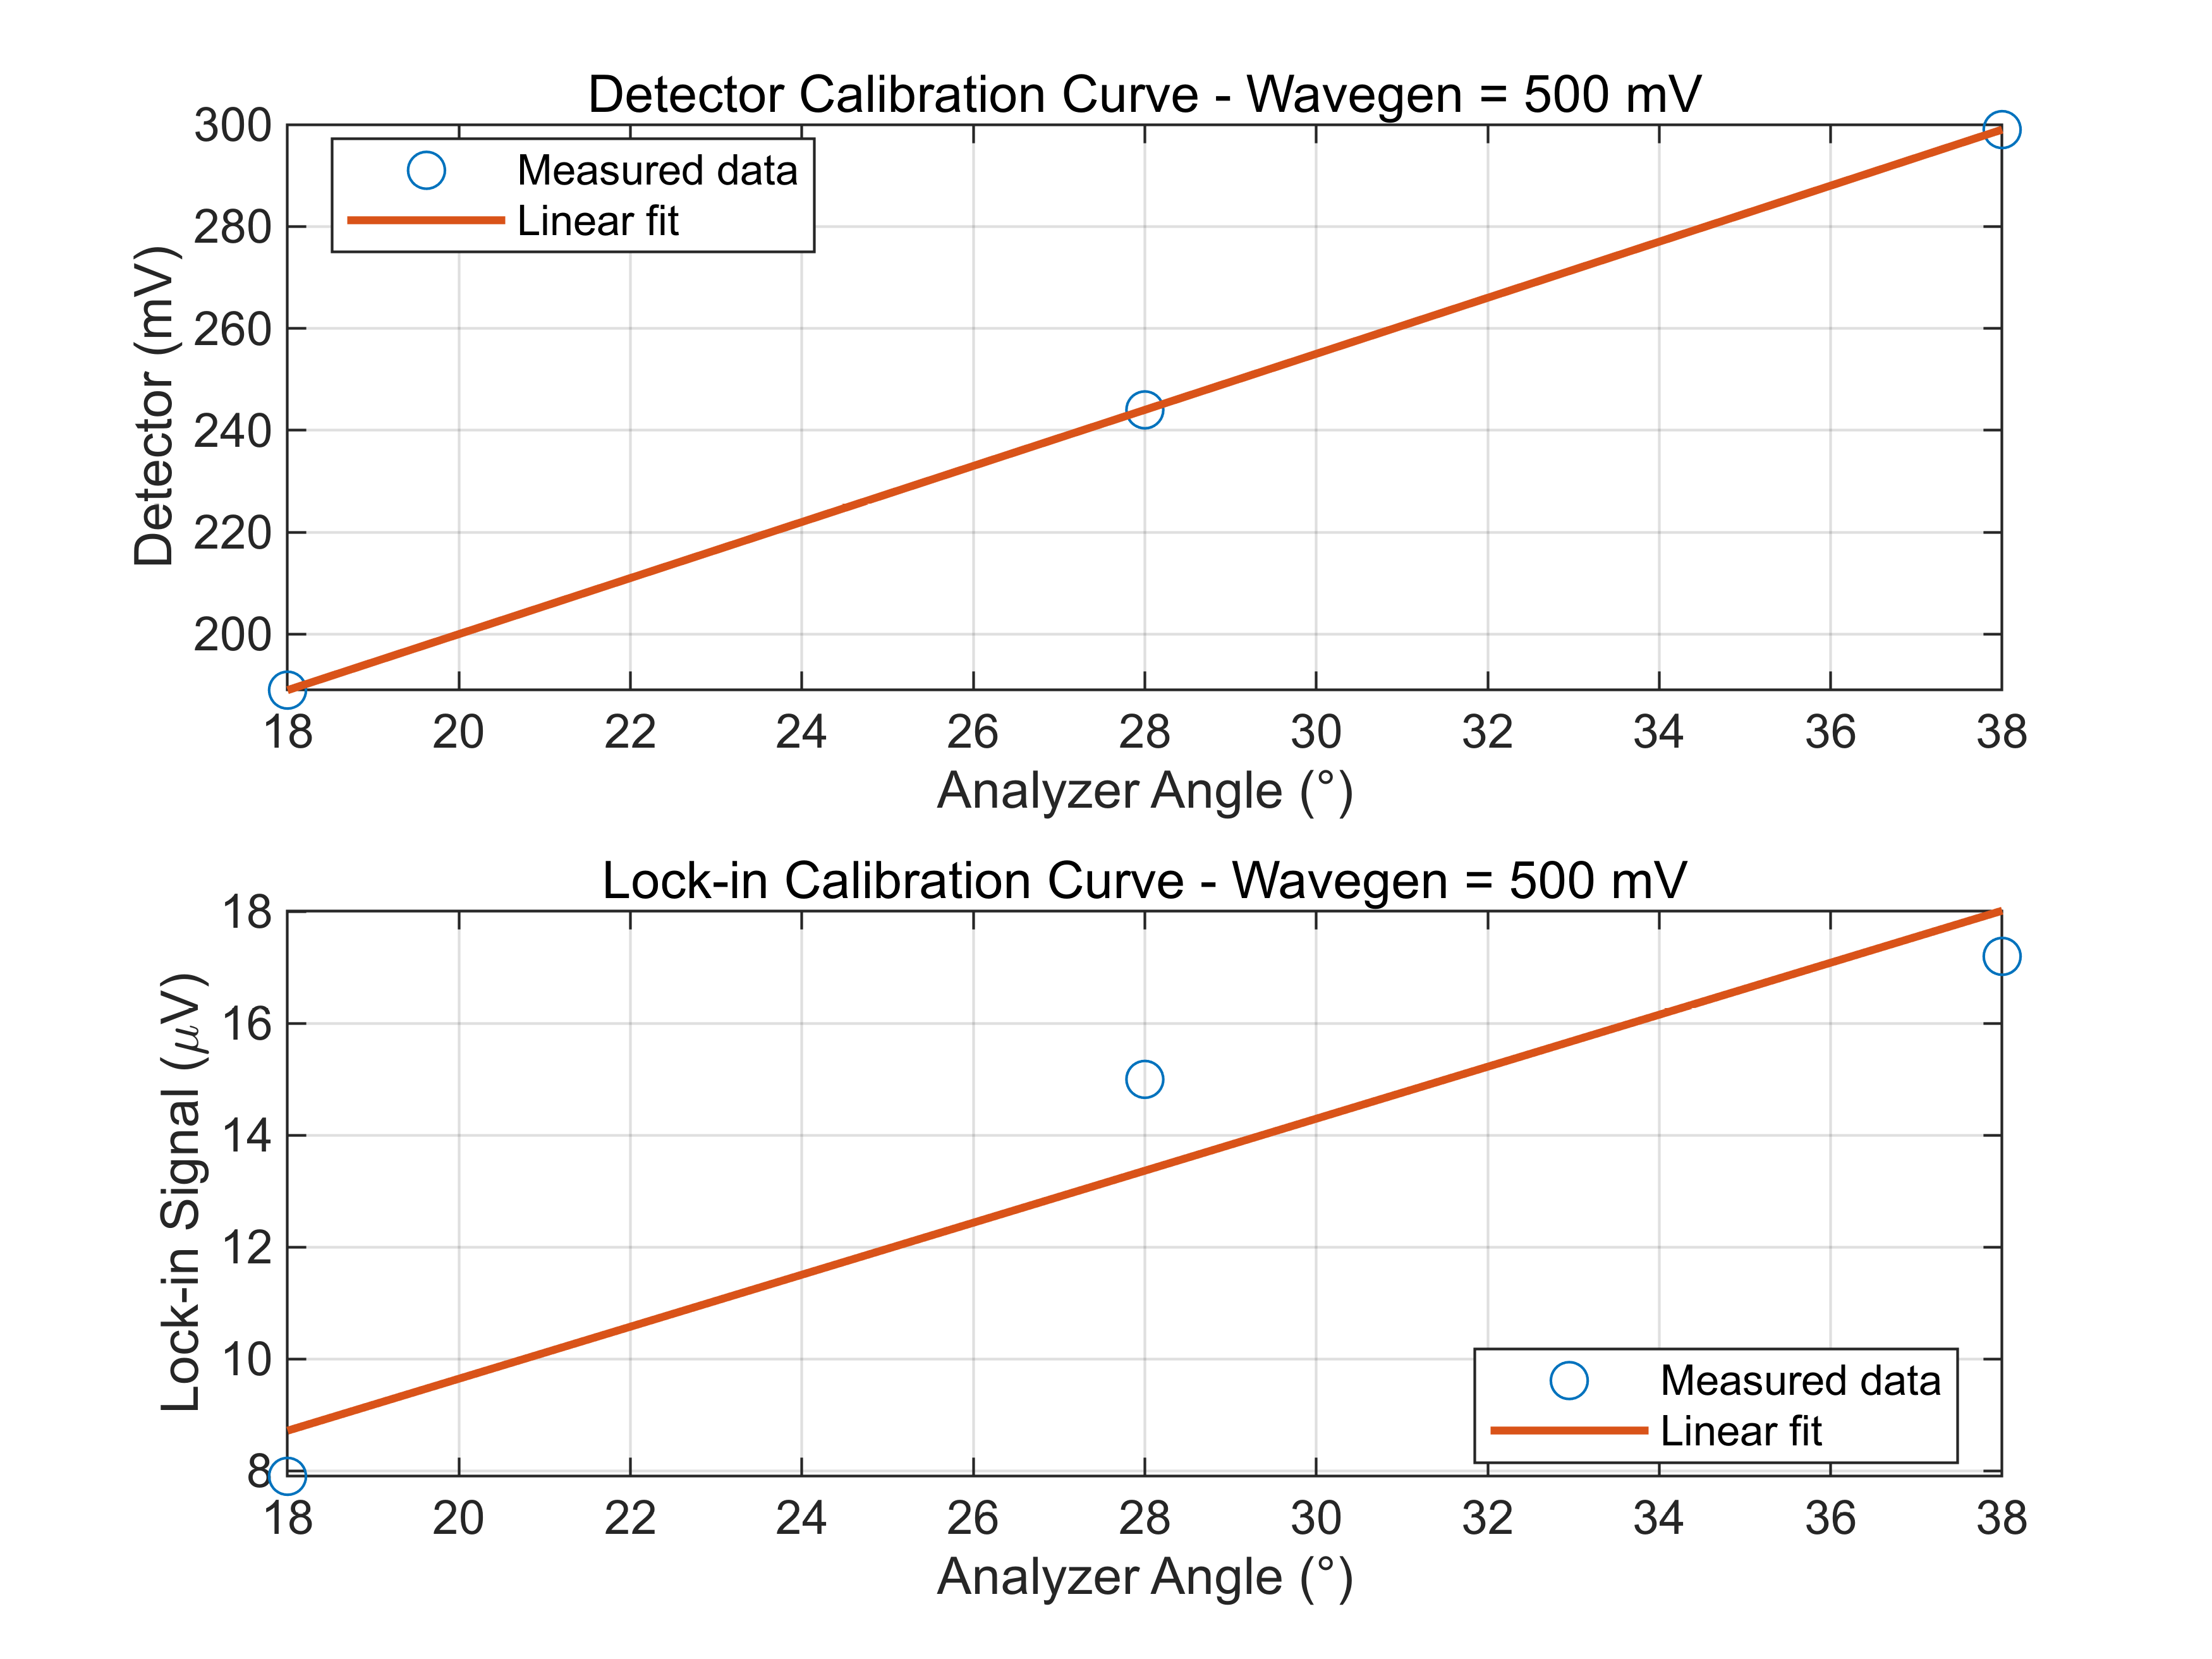
\includegraphics[width=\linewidth]{5.2.png}
        \caption*{b) 500 mV}
    \end{minipage}\hfill
    \begin{minipage}{0.5\textwidth}
        \centering
        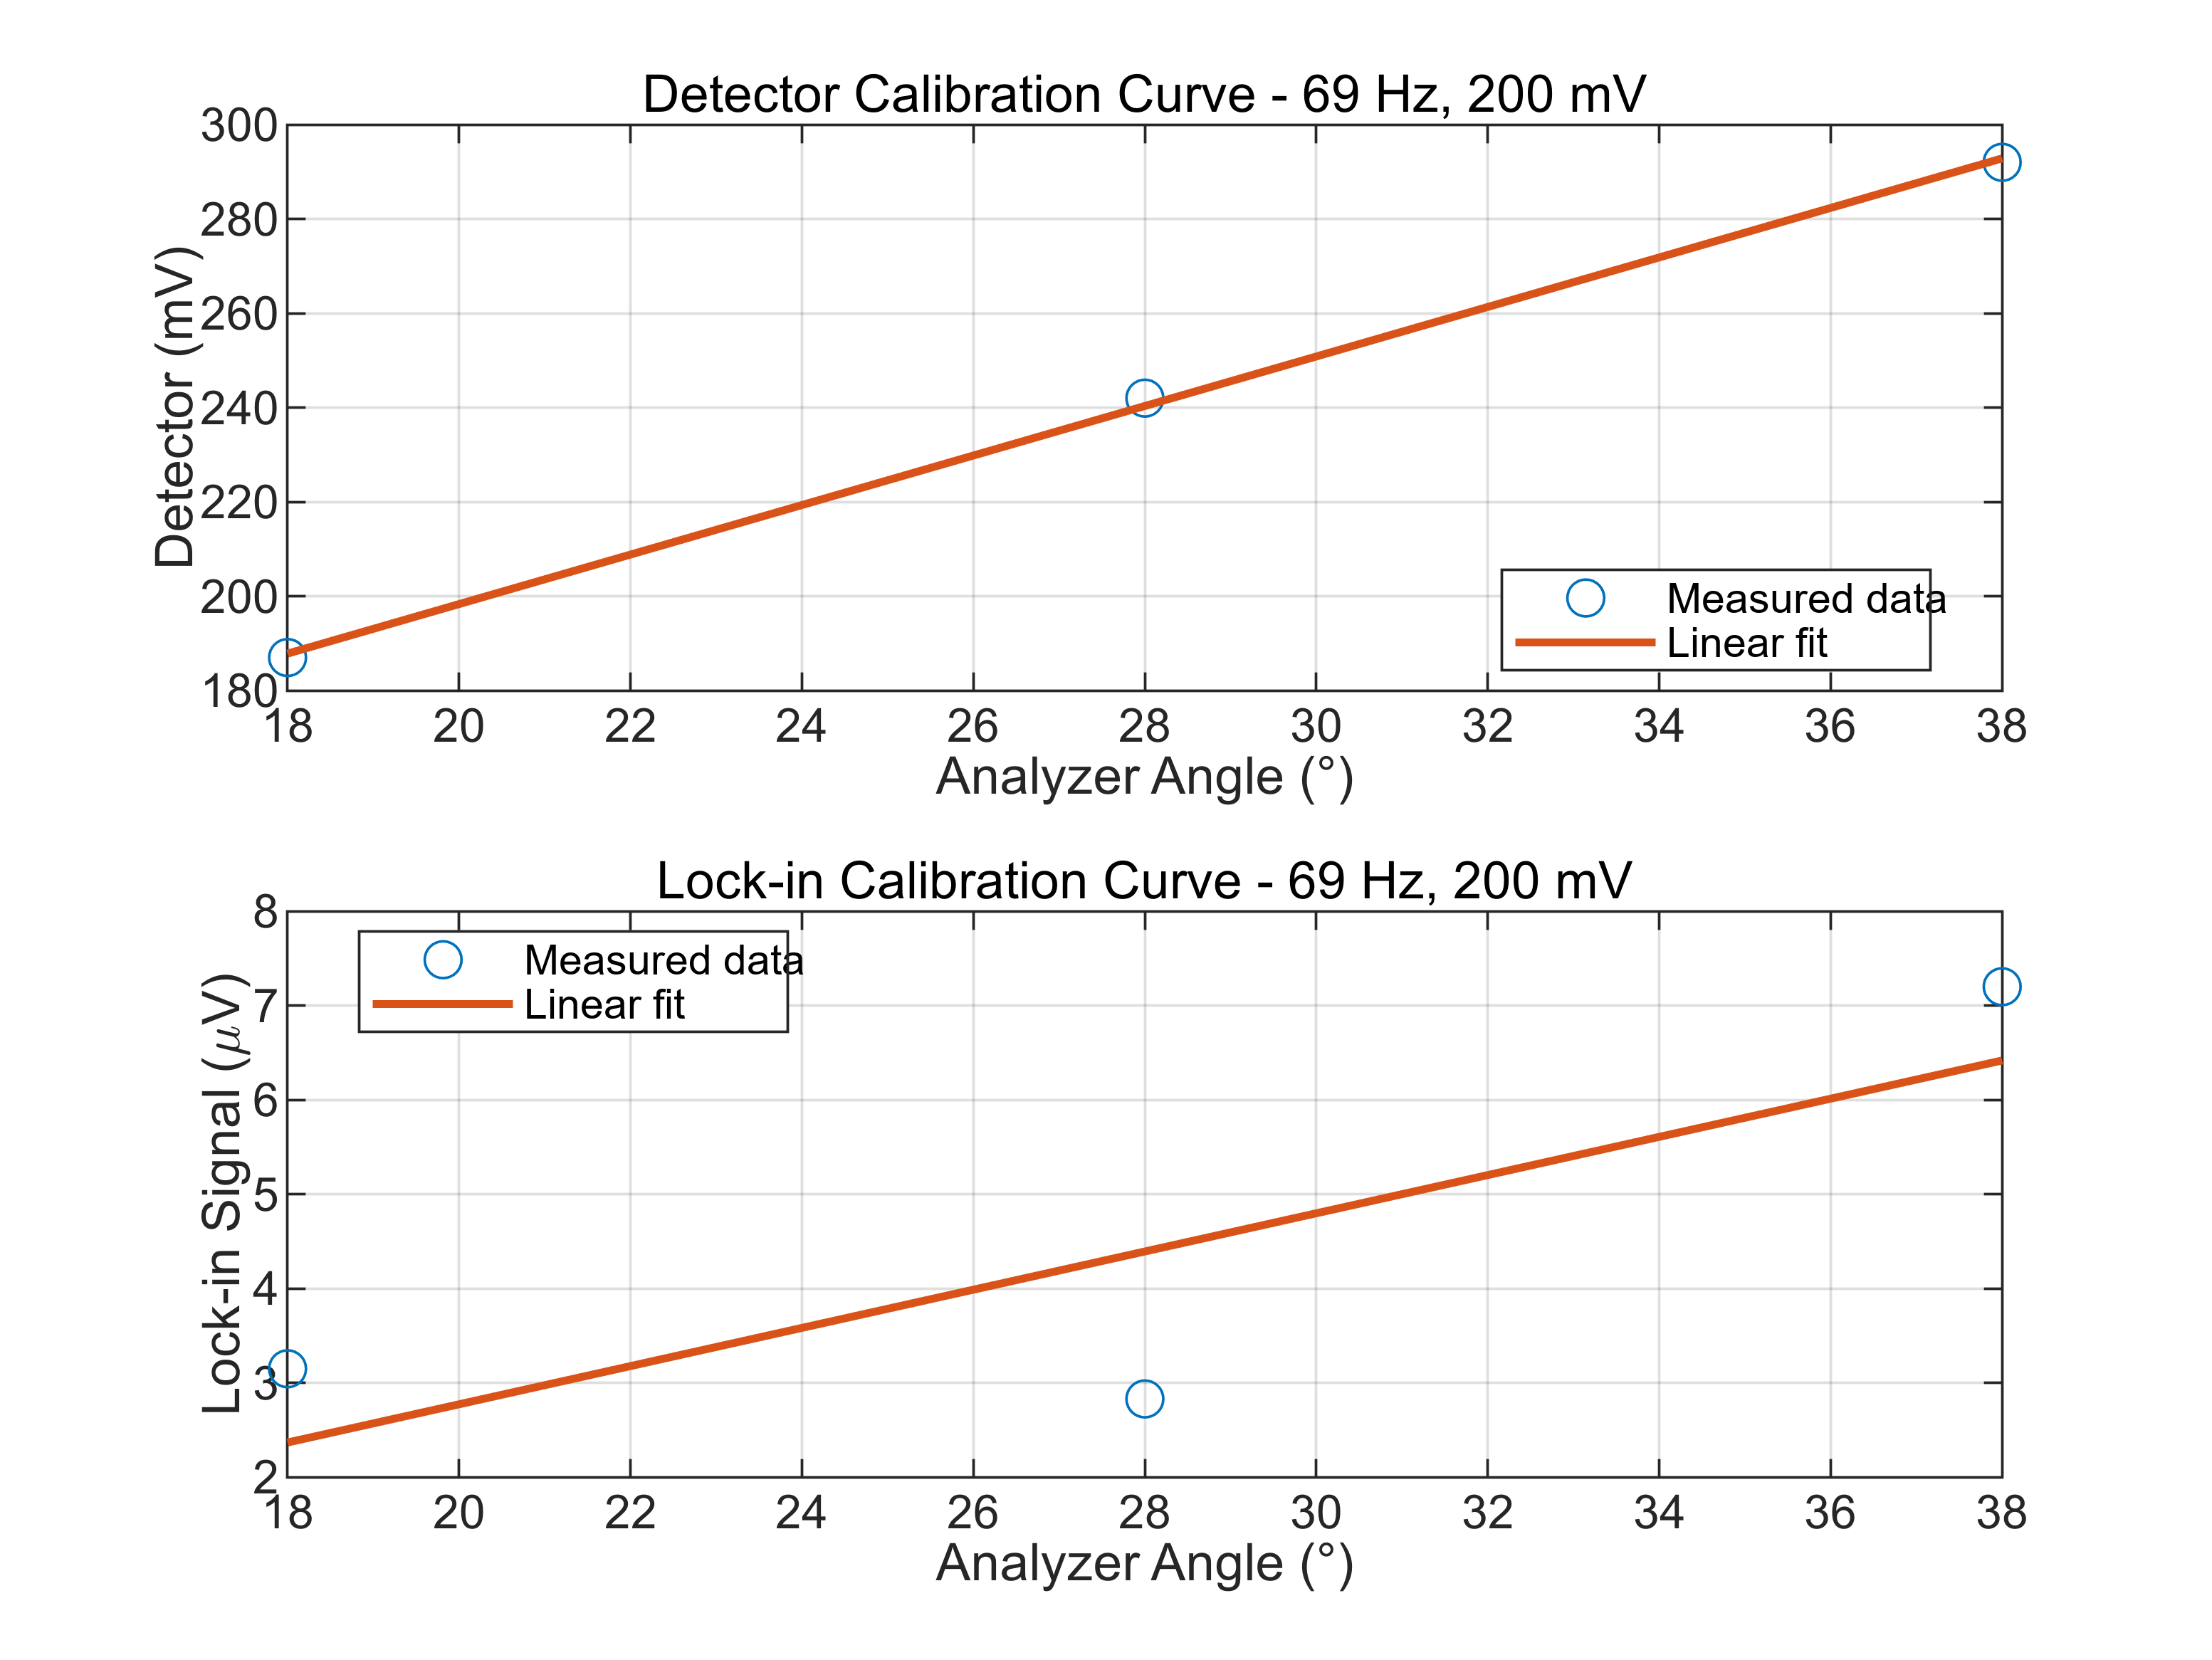
\includegraphics[width=\linewidth]{5.3.png}
        \caption*{c) 200 mV, 69 Hz}
    \end{minipage}
    \caption{Calibration plots of detector and lock-in responses vs. analyzer angle under three different modulation settings with linear fitting}
    \label{fig:task5_calibration}
\end{figure}





\subsection{Tasks 6 \& 7: Magneto-Optical Detection and Concentration Dependence of Hemozoin}

\textbf{Objective.}
The goal of these tasks was to measure the linear dichroism of synthetic hemozoin suspensions under varying magnetic field orientations and to investigate how different hemozoin concentrations affect the detected optical signal.

\textbf{Procedure.}
The sample holder was inserted into the light path, and measurements were performed using the previously determined optimal modulation setting of \(200\,\mathrm{mV}\) at \(20\,\mathrm{Hz}\). The DC detector signal and the lock-in amplifier signal were recorded first with the magnetic field in a vertical orientation, and then the magnet was rotated by \(90^\circ\) to a horizontal orientation. This procedure was repeated across three different cuvettes: distilled water (0\% hemozoin), a 5\% hemozoin suspension, and a denser 10\% hemozoin suspension.

\textbf{Results.}
The measured signals for the different concentrations were:
\begin{itemize}
    \item \textbf{0\% Hemozoin (Distilled Water):}
    \begin{itemize}
        \item Vertical Magnetic Field: Detector = \(400.10\,\mathrm{mV}\), Lock-In = \(2.91\,\mu\mathrm{V}\)
        \item Horizontal Magnetic Field: Detector = \(400.20\,\mathrm{mV}\), Lock-In = \(5.00\,\mu\mathrm{V}\)
    \end{itemize}
    \item \textbf{5\% Hemozoin:}
    \begin{itemize}
        \item Vertical Magnetic Field: Detector = \(70.30\,\mathrm{mV}\), Lock-In = \(1.94\,\mu\mathrm{V}\)
        \item Horizontal Magnetic Field: Detector = \(86.40\,\mathrm{mV}\), Lock-In = \(2.41\,\mu\mathrm{V}\)
    \end{itemize}
    \item \textbf{10\% Hemozoin:}
    \begin{itemize}
        \item Vertical Magnetic Field: Detector = \(29.00\,\mathrm{mV}\), Lock-In = \(5.41\,\mu\mathrm{V}\)
        \item Horizontal Magnetic Field: Detector = \(38.65\,\mathrm{mV}\), Lock-In = \(4.32\,\mu\mathrm{V}\)
    \end{itemize}
\end{itemize}

\begin{figure}[H]
    \centering
    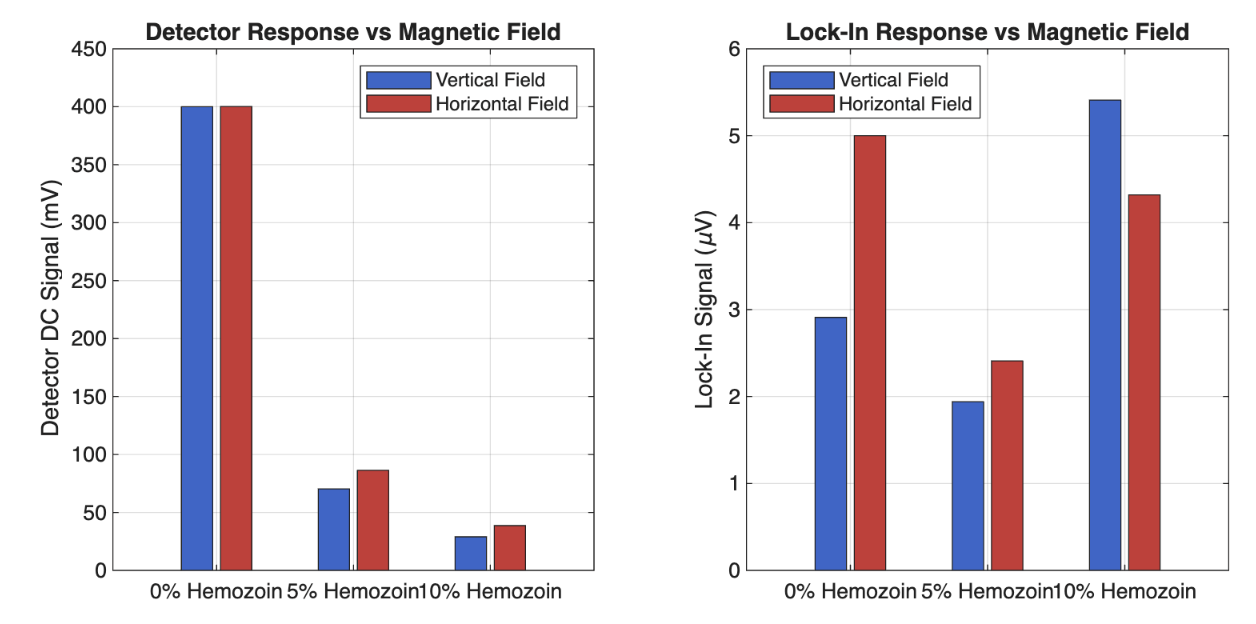
\includegraphics[width=0.8\linewidth]{t67_hemozoin_plot.png}
    \caption{Comparison of Detector DC signal and Lock-In response for 0\%, 5\%, and 10\% hemozoin concentrations under vertical and horizontal magnetic fields.}
    \label{fig:task67_comparison}
\end{figure}


The plotted data (See Figure \ref{fig:task67_comparison}) reveals both the magneto-optical effect and a clear concentration dependence. The sub-micron hemozoin crystallites align when placed in an external magnetic field. Due to their low symmetry, an optical anisotropy appears for linear polarization along and perpendicular to the magnetic field. When the field is rotated by \(90^\circ\), the orientation of the crystals changes accordingly, altering this optical anisotropy and significantly affecting the measured transmitted signal.

This effect is isolated by comparing the samples. In the absence of hemozoin crystals (0\%), a change in the magnetic field orientation does not induce optical anisotropy, leaving the DC detector signal almost perfectly constant (\(400.10\,\mathrm{mV}\) vs \(400.20\,\mathrm{mV}\)). Conversely, as the hemozoin concentration increases to 5\% and then 10\%, the overall optical transmission decreases significantly (dropping from \(400\,\mathrm{mV}\) down to the \(29\)--\(86\,\mathrm{mV}\) range) due to higher absorption and scattering. Despite these optical losses, the suspensions containing hemozoin clearly exhibit the characteristic signal shift upon field rotation, successfully demonstrating the magneto-optical detection of the crystals.








\section{Summary}

The basic characterization of the film polarizers verified Malus' law and yielded an extinction ratio of \(1.33 \times 10^{-3}\), which aligns well with expected commercial standards for dichroic polarizers\cite{thorlabs_film_polarizers}. While evaluating the zero-voltage state of the liquid crystal cell, we found that it produced an elliptical polarization state rather than the ideal \(\pi/2\) retardation, allowing us to calculate a baseline retardation of \(\approx 128^\circ\) and an optical path-length difference of \(\approx 231\,\mathrm{nm}\).

By utilizing a continuous amplitude sweep, we mapped the voltage-dependent retardation \(\delta(V)\) of the LC cell. The measured transmission curves for the parallel and crossed configurations were nearly perfectly complementary (\(T_\parallel + T_\perp \approx 0.98\)), accurately reflecting the theoretical threshold and boundary pinning dynamics of nematic liquid crystals. 

Finally, after identifying the \(200\,\mathrm{mV}\) at \(20\,\mathrm{Hz}\) modulation setting as the optimal balance of sensitivity and signal purity, the setup successfully detected synthetic hemozoin. While the 0\% control sample showed no response to magnetic field changes, the 5\% and 10\% suspensions exhibited distinct transmission shifts when the magnetic field was rotated by \(90^\circ\). This confirmed the magneto-optical alignment of the paramagnetic crystallites and successfully validated the polarization-modulation setup as a viable diagnostic method for malaria pigment.







\begin{thebibliography}{9}
    \bibitem{lab_notes} \textit{Notes for students about Laboratoires.pdf}.
    \bibitem{lab_desc} \textit{Magneto (2).pdf}. Specialization Laboratory Measurement 2: Light polarization modulation using a liquid crystal cell: detection of malaria pigment. 
    \bibitem{thorlabs_film_polarizers} Thorlabs. (n.d.). \textit{Economy Film Polarizers}. Retrieved from \texttt{https://www.thorlabs.com/economy-film-polarizers}.
\end{thebibliography}

\end{document}
